\section{State-Of-The-Art Analyse}

\subsection{Betrachtungsgegenstand}
Der derzeitige State-Of-The-Art im Bereich \ac{T2P} ist das Verfahren von Friedrich aus dem Jahr 2011 (\cite[vgl.][11]{RIEFER}). Im Folgenden wird die von Friedrich erarbeitete Vorgehensweise (\cite[vgl.][11]{FRIEDRICH1} und \cite[vgl.][11]{FRIEDRICH2}) analysiert und Verbesserungsvorschläge erarbeitet.
Die Analyse beschränkt sich auf die Textverarbeitung bishin zur generierung des World Models. Die Konstruktion eines Graphen aus dem World Model ist nicht Teil dieser Arbeit.
\par
Zunächst wird im Folgenden kurz auf den konkreten Aufbau des World Models nach Friedrich eingegangen. Anschließend folgt die Analyse der Vorgehensweise. Gemäß der durch Friedrich vorgegebenen Gliederung wird zunächst die Textverarbeitung auf Satz-Ebene und dann die Textverarbeitung auf Text-Ebene analysiert. Abschließend werden bekannte Problemfelder zusammengetragen und Lösungsansätze vorgeschlagen.

\subsection{World Model}
World Model: Actor, Resource, Action, Flow
Enrichment of Worldmodel step by step
(= Ziel)

\subsection{Textverarbeitung auf Satz-Ebene}

Der Eingangstext in natürlicher Sprache wird zunächst in einzelne Wörter und Sätze aufgesplittet. In \ref{fig:SLEVEL} wird dieser Vorgang der \textit{Sentence Decomposition} zugeordnet. Es handelt sich hierbei um eine normale Tokenization, bei der auf die Stanford CoreNLP Funktionen \textit{Stanford TokenizerAnnotator} und \textit{Stanford WordsToSentenceAnnotator} zurückgegriffen wird. Im nächsten Schritt wird der Text mit dem \textit{POSTaggerAnnotator} mit \textit{POS-Tags} versehen und anschließend mit dem PCFG-Parser \textit{ParserAnnotator} die Satzstruktur analysiert. Dies wird durch den Pfeil von StanfordParser zu Subprozess in \ref{fig:SLEVEL} symbolisiert. Auf eine pauschale \textit{Lemmatization} aller Wörter wird an dieser Stelle verzichtet.

\begin{wrapfigure}{r}{13cm}
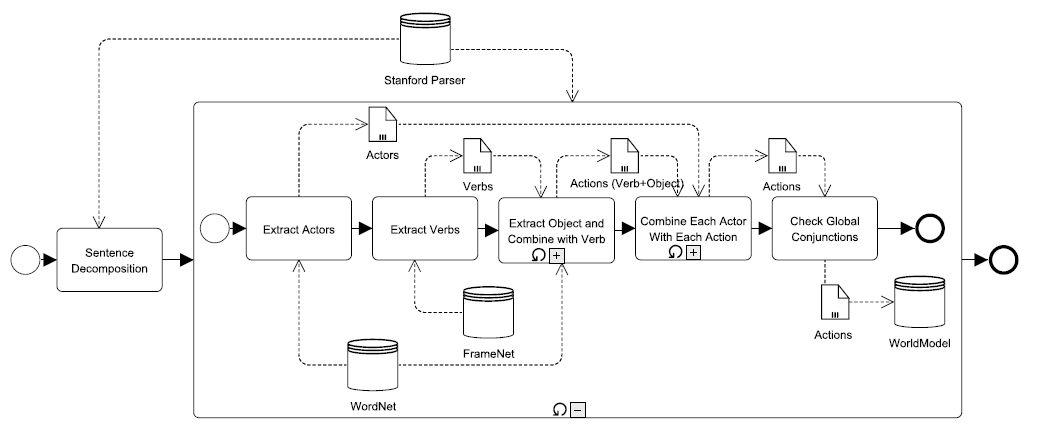
\includegraphics[width=13cm]{pictures/SentenceLevel.png}
\caption{Analyseschema auf Satzebene (\cite[vgl.][5]{FRIEDRICH2})}
\label{fig:SLEVEL}
\end{wrapfigure}

Auf Basis der Annotationen folgt dann das \textit{Phrase Chunking}, der zweite Teil der Sentence Decomposition. Die annotierten Informationen...




Algorithm phrase chunking (problem of complex sentences)
- check if active or passive (Active-passive issue)
- Actors and actions are extracted and filtering (example sentences filtered out with stop word list)
-->SRL Task
- combining each action with each object
- same with actors, action has to be atomic
- all are added to world model

Step 2 Text Level Analysis:
- taking sentence relationships into account
- resolve relative references in text (anaphora relolution algorithm issue 4.1)
- conditional markers (based on 4 lists, AI?)
combine info in different actions (2.2) wich are split over sentences
- dafür: merger candidates with anaphora resolution
- textua links: 3 typen von links forwärts, rückwärts und jumper
- vergleich übe root form
-last step: Flow generation
- bisher nur or, and/or und and


Thesis:
Anaphora resolution:
pronouns, determiners, relative pronouns ok. Problem: Steve Jobs = CEO of Apple

Semantic Role Labelling
Extract Actor, Resource, Actions, Flows

1) Decomposition (Tokenization)
2) Parsing

issue cathegories: Syntactic Leeway, Atomiticity, Relevance, Referencing
--> Classic NLP tasks

\subsection{Textverarbeitung auf Text-Ebene}
\subsection{Problemfelder und Lösungsansätze}



